\chapter{Per cominciare}\label{cha:install}


\section*{Obiettivi di apprendimento}

Lo studio di questo capitolo dovrebbe insegnare allo studente come:
\begin{itemize}
\item 
  Installare \R\, e RStudio.
\end{itemize}


\section*{Motivazione}

Al fine di utilizzare \R\, è necessario eseguire le seguenti tre operazioni nell'ordine dato:
\begin{enumerate}
\item Installare \R;
\item Installare RStudio;
\item Installare \R-Packages (se necessario).
\end{enumerate}
Vedremo qui come installare \R\, e RStudio.


\section{Installare \R\, e RStudio}

\R\, è disponibile gratuitamente ed è scaricabile dal sito \url{http://www.rproject.org/}. 
Dalla pagina principale del sito \verb+r-project.org+ andiamo sulla sezione \verb+Download+ e scegliamo un server a piacimento per scaricare il software d'installazione. 
Una volta scaricato l'installer, lo installiamo come un qualsiasi software, cliccando due volte sul file d'istallazione. 
Esistono versioni di \R\, per tutti i più diffusi sistemi operativi (Windows, Mac OS X e Linux).
%\footnote{
%È possibile che, dopo l'installazione di \R\, sul Mac, nella console di \R\, compaia il seguente messaggio: 
%\texttt{Warning messages: Setting LC\_CTYPE failed, using C...}
%Per correggere questo problema, aprite il terminale di Mac e digitate la seguente stringa: 
%\texttt{defaults write org.R-project.R force.LANG en\_US.UTF-8}
%Si può poi chiudere il terminale di Mac e fare ripartire \R. 
%}

Il \R\, Core Development Team lavora continuamente per migliorare le prestazioni di \R\,, per correggere errori e per consentire l'uso di \R\, con nuove tecnologie.  
Di conseguenza, periodicamente vengono rilasciate nuove versioni di \R. 
Informazioni a questo proposito sono fornite sulla pagina web \url{https://www.r-project.org/}. 
Per installare una nuova versione di \R\, si segue la stessa procedura che è stata seguita per la prima installazione.
\footnote{
Insieme al software si possono scaricare dal sito principale sia manuali d'uso che numerose dispense per approfondire diversi aspetti di \R. 
In particolare, nel sito \url{http://cran.r-project.org/other-docs.html} si possono trovare anche numerose dispense in italiano (sezione ``Other languages'').
}

Dopo avere installato \R\, è opportuno installare anche RStudio.
RStudio si può scaricare da \url{https://www.rstudio.com/}.
Anche RStudio è disponibile per tutti i più diffusi sistemi operativi.


\section{Utilizzare RStudio per semplificare il lavoro}

Possiamo pensare ad \R\, come al motore di un automobile e a RStudio come al cruscotto di un automobile.
Più precisamente, \R\, è un linguaggio di programmazione che esegue calcoli mentre RStudio è un ambiente di sviluppo integrato (IDE) che fornisce un'interfaccia grafica aggiungendo una serie di strumenti che facilitano la fase di sviluppo e di esecuzione del codice.
Utilizzeremo dunque \R\, mediante RStudio.
In altre parole, 
\begin{figure}[h!]%
\captionsetup[subfigure]{labelformat=empty}
    \centering
    \subfloat[\textbf{non aprite}]{{
\includegraphics[width=2.35cm]{R_logo}}}%
    \qquad\qquad\qquad\qquad
    \subfloat[\textbf{aprite}]{{
\includegraphics[width=5cm]{RStudio-Logo-Blue-Gradient}}}%
    %\caption{2 Figures side by side}%
    %\label{fig:example}%
\end{figure}

L'ambiente di lavoro di RStudio è costituito da quattro finestre (Figura~\ref{fig:rstudio_pics}):
 la finestra del codice (scrivere-eseguire script),
 la finestra della console (riga di comando - output),
la finestra degli oggetti (elenco oggetti-cronologia dei comandi) e
la finestra dei pacchetti-dei grafici-dell'aiuto in linea.

\begin{figure}[h!]
\centering
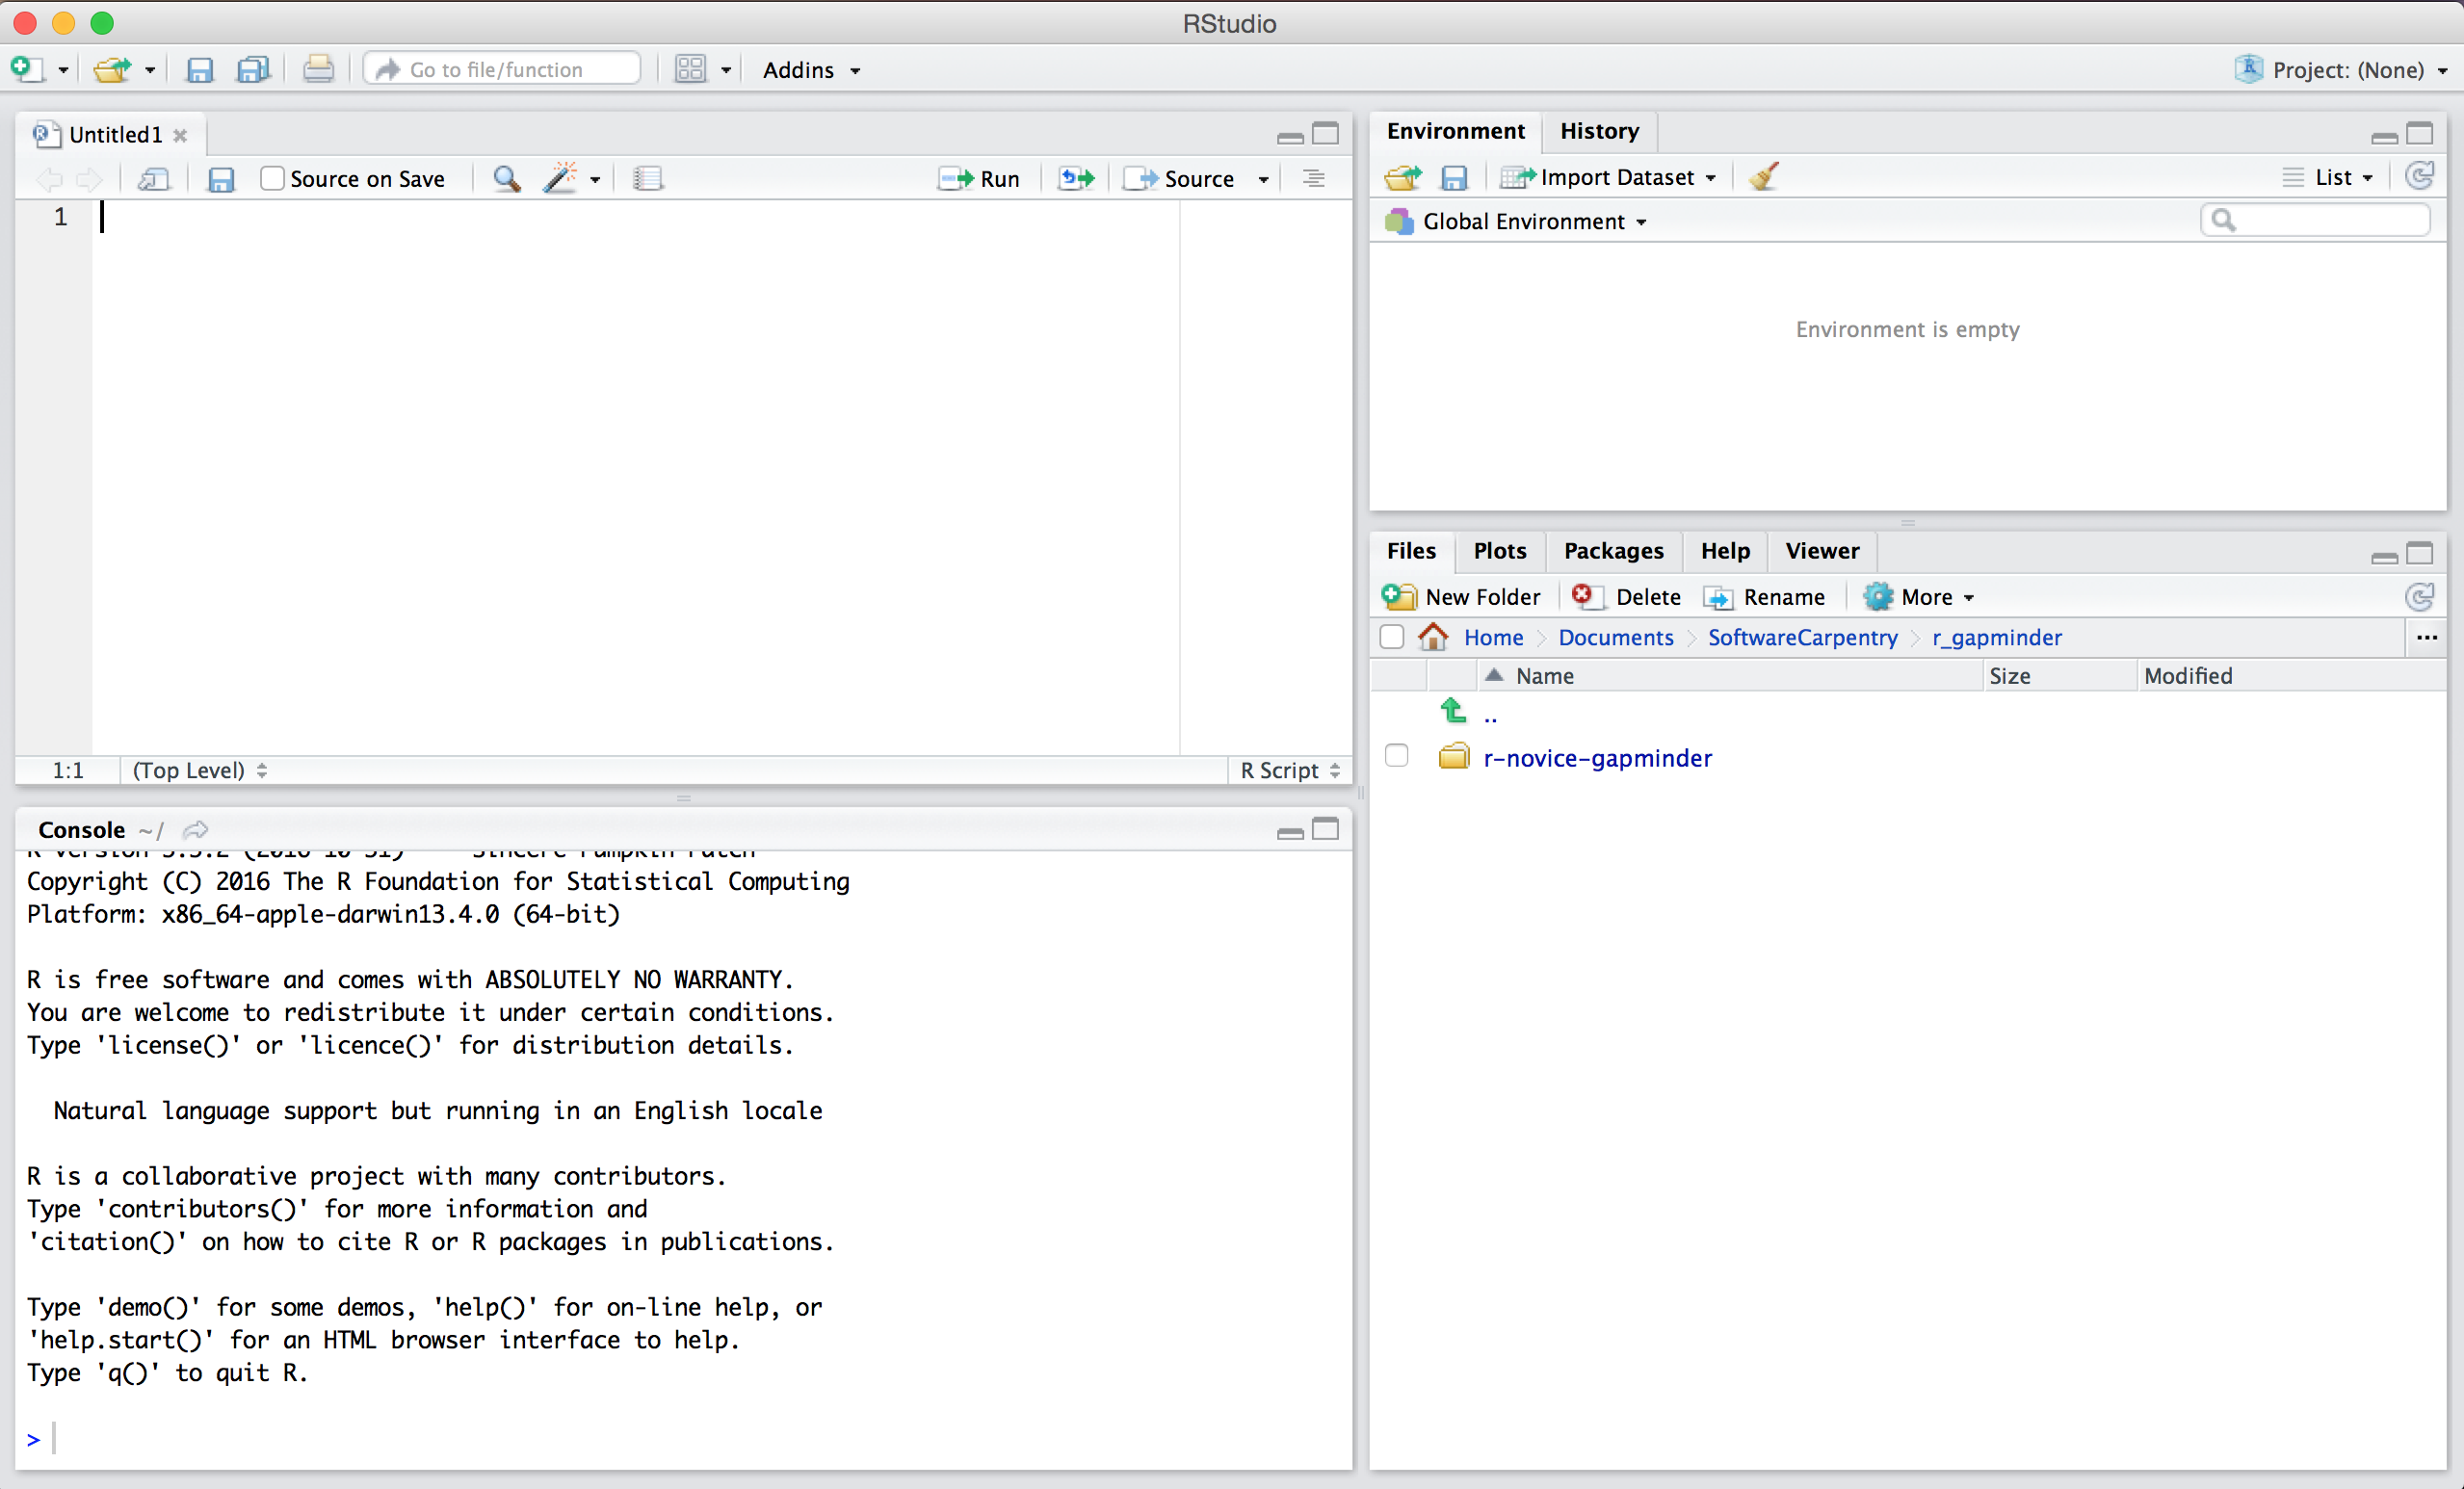
\includegraphics[width=\textwidth]{rstudio_pics}
\caption{La console di RStudio.}
\label{fig:rstudio_pics}
\end{figure}


\subsection{Eseguire il codice}

Mediante il menu a tendina di RStudio, scegliendo il percorso 
\begin{lstlisting}
File > New File > R Notebook
\end{lstlisting}
oppure 
\begin{lstlisting}
File > New File > R Script
\end{lstlisting}
l'utente può aprire nella finestra del codice (in alto a destra) un \R\, Notebook o un \R\, script  dove inserire le istruzioni da eseguire.

In un \R\, script, un blocco di codice viene eseguito selezionando un insieme di righe di istruzioni e digitando la sequenza di tasti \verb|Command| + \verb|Invio| sul Mac, oppure \verb|Control| + \verb|Invio| su Windows.
In un \R\, Notebook, un blocco di codice viene eseguito schiacciando il bottone con l'icona  $ \color{red}\blacktriangleright$ (\enquote{Run current chunk}) posizionata a destra rispetto al codice.



